\section{Accuracy estimation for retraining configurations}
\label{sec:profiling}

% profiling problem definition 
As shown in Figure \ref{fig:sys-arch} and explained in \S\ref{sec:solution}, {\name} relies on estimated accuracies of the retraining configurations for its scheduling decisions for each retraining window. Specifically, at the beginning of each retraining window $w$, the thief scheduler requires the estimated accuracy of each configuration $\gamma_v$, denoted as $a_v^{(w,\gamma)}$. The resource demands of the retraining configurations scale well with the size of the training data, and thus they only need to be measured once.

% history vs. current window
We consider two broad approaches to estimating the accuracy, $a_v^{(w,\gamma)}$. The first approach is {\em online} where a ``profiler'' is executed on a sub-sample of the training data on all candidate configurations \cite{videostorm}. However, this approach is time-consuming and strains the already resource-constrained edge server. Instead, we use {\em history} and predict the accuracy using accuracy values from prior retraining windows.

% history; class distribution 
History-based profiling is widely used to optimize machine-learning systems (\eg~\cite{awstream,chameleon}). 
A natural approach is to predict $a_v^{(i,\gamma)}$ using a moving-window average over a history of $k$ retraining windows, $a_v^{(i-1,\gamma)},a_v^{(i-2,\gamma)},\dots,a_v^{(i-k,\gamma)}$ where $\gamma$ is the retraining configuration. The main drawback with this approach is that it mixes accuracy values from windows with different class distributions. A better approach, instead, is to use only those prior windows whose class distributions are similar to the current window. We use the Euclidean distance as our measure of similarity between class distributions. %It aggregates the accuracy values from similar history windows, grouped by individual configurations. 


%\begin{figure}[t!]
%\centering
%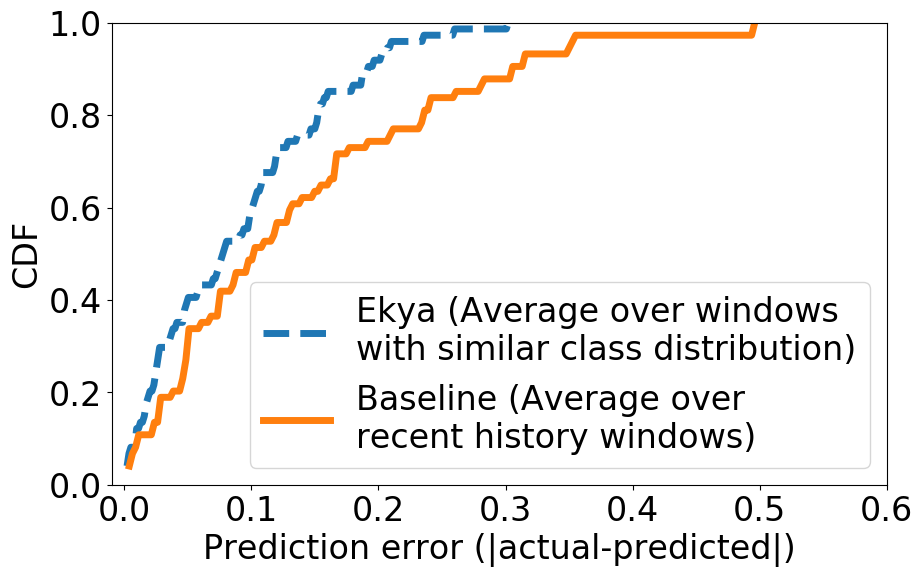
\includegraphics[width=0.8\columnwidth]{figures/eval_placeholders/cdf-profiler-error.png}
%\vspace{-0.2cm}
%\caption{\name's profiler can predict the model accuracy after retraining with less error than the baseline of moving average over recent history windows.\zhengxu{pdf file added. change filename in tex when needed}\romil{We should pdf this}
%\vspace{-0.2cm}}
%\label{fig:profiler-error}
%\end{figure}


% insight
Given the inherent tradeoff between compressing models (for efficiency) and their generalizability (\S\ref{subsec:continuous}), the closer the distribution of classes is between two retraining windows, the similar the accuracies are of the models retrained in those windows. Our evaluations of the above simple predictor on the different video datasets from Cityscapes and Waymo (\S\ref{subsec:eval-setup}) show that our prediction (of accuracy) is nearly $10\%$ points better at the median (and $18\%$ points at the $90^\text{th}$ percentile).%; see Figure \ref{fig:profiler-error}.  
%The insight is that the accuracy of a retrained model depends more on difficulty of the data used to retrain the model. For instance, if the training data consist of only a handful of classes, the retrained model can be very high accurate since the data have low complexity. Otherwise, if the training data include tens of classes, the retrained model will tend to have slightly lower accuracy on each class, due to the inherent capacity/complexity tradeoff of cheap DNN models. In other words, if two retraining windows are comprised of similar distribution of classes, the retraining accuracies tend to similar. (Of course, there can be other metric of difficulty of the training data than class distribution, but we empirically found class distribution works well in our setting.)
% \gaa{We should stress that even if two windows have similar class distributions, it does not mean the retrained model from one window can be re-used in the other due to discrepancies in other aspects (camera lighting, angles of objects, etc; \S\ref{subsec:continuous-measurement}).}

We should stress that even if two windows have similar class distributions, it merely means the two windows are equivalent in their difficulty to reach high accuracy through retraining; it does {\em not} mean the retrained model from one window can be re-used in the other (as \S\ref{subsec:continuous-measurement} showed, other factors such as lighting and angles of objects may be considerably different between the two windows). We show the degraded accuracy of such a solution that caches and uses past models from windows with similar class distributions in \S\ref{subsec:eval-alternate}.
% due to discrepancies in other aspects (camera lighting, angles of objects, etc; \S\ref{subsec:continuous-measurement}).

% no history available 
When there is no retraining window in history with similar distributions for the configuration $\gamma$, {\name} resorts to the online approach. It retrains using $\gamma$ on a small fraction of the training data. The accuracy from these runs are provided to Algorithm \ref{algo:thief_sched}. \name seldom has to resort to the online approach since it looks sufficiently long back in history. 
%For instance, one can try several retraining configurations in parallel on a small subsample of the training data. In the case when there is no history window with similar class distribution that used the queried retraining configuration, by default \name will apply the configuration to retrain the model (if there is enough resource).
% exploration phase; exhaustive profiling to identify promising configurations 
To build a rich history, \name periodically opts for a randomly chosen configuration (from the Pareto boundary) in its retraining. Such an approach of ``exploration'' allows it to build a mapping between data distributions, configurations, and their accuracy values. 

{\bf Training labels.} Note that for the current retraining window as well as for the historical windows, {\name} acquires ``ground-truth'' labels using a golden model -- a high-cost but high-accuracy model pre-trained on a large dataset -- consistent with prior work \cite{incremental-13, mullapudi2019, incremental-15, distribution-20}. In every retraining window, {\name} runs the golden model on the training data to generate labels for retraining. We use the ResNet152 model trained on the MS-COCO dataset as our golden model. The cost of running the golden model is typically small (measured to be under $3\%$ of the retraining cost, as per our experiments).
% \romil{Add experiment to justify that golden model outputs are indeed representative of the ground truth}


% empirical numbers
%To show the effectiveness of our idea, Figure~\ref{fig:profiler-error} picks a retraining configuration (retraining last layer of ResNet18) and compares the prediction error of two strategies per Waymo retraining window: running average over recent four history windows (baseline) and average over windows with similar class distributions (\name's profiler).\footnote{Notice that this is an idealized assumption; \name will not have a measured accuracy of the same configuration in all history windows, but the fact that our method based on class distribution similarity uses less windows, so in practice, our prediction can be even more accurate than the baseline.} To identify retraining windows that have similar class distribution, we group the class distributions into 5 clusters which acount for 70\% of retraining windows. We see that \name has on average 10\% lower prediction errors (with more reduction on the high percentiles). We should stress that even if two windows have similar class distributions, it does not mean the retrained model from one window can be re-used in the other due to discrepancies in other aspects (camera lighting, angle, etc).

